\chapter{Kvalitativt interview}
\label{appendix:interview}
\section{Interview guide}
\begin{figure}
    \centering
    
\includegraphics[width=\textwidth]{Images/appendixB/1.jpg}
    \caption{Kvalitativt interview guide — Del 1}
    \label{img:appendixc:1}
\end{figure}

\begin{figure}
    \centering
    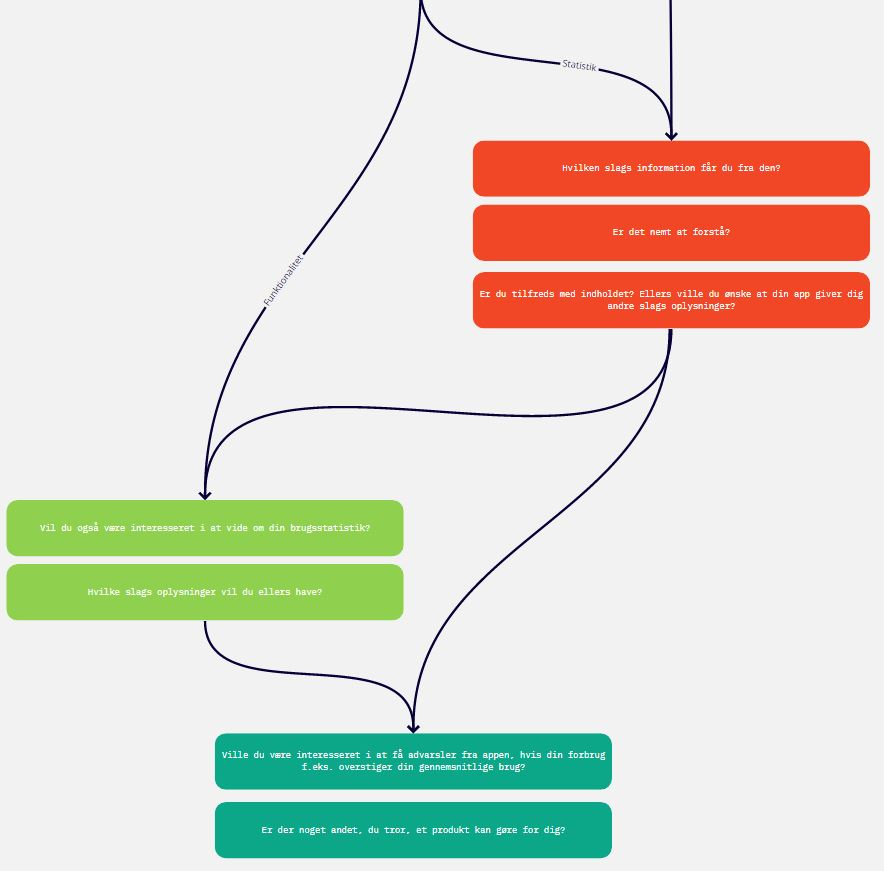
\includegraphics[width=\textwidth]{Images/appendixB/2.jpg}
    \caption{Kvalitativt interview guide — Del 2}
    \label{img:appendixc:2}
\end{figure}

\begin{figure}
    \centering
    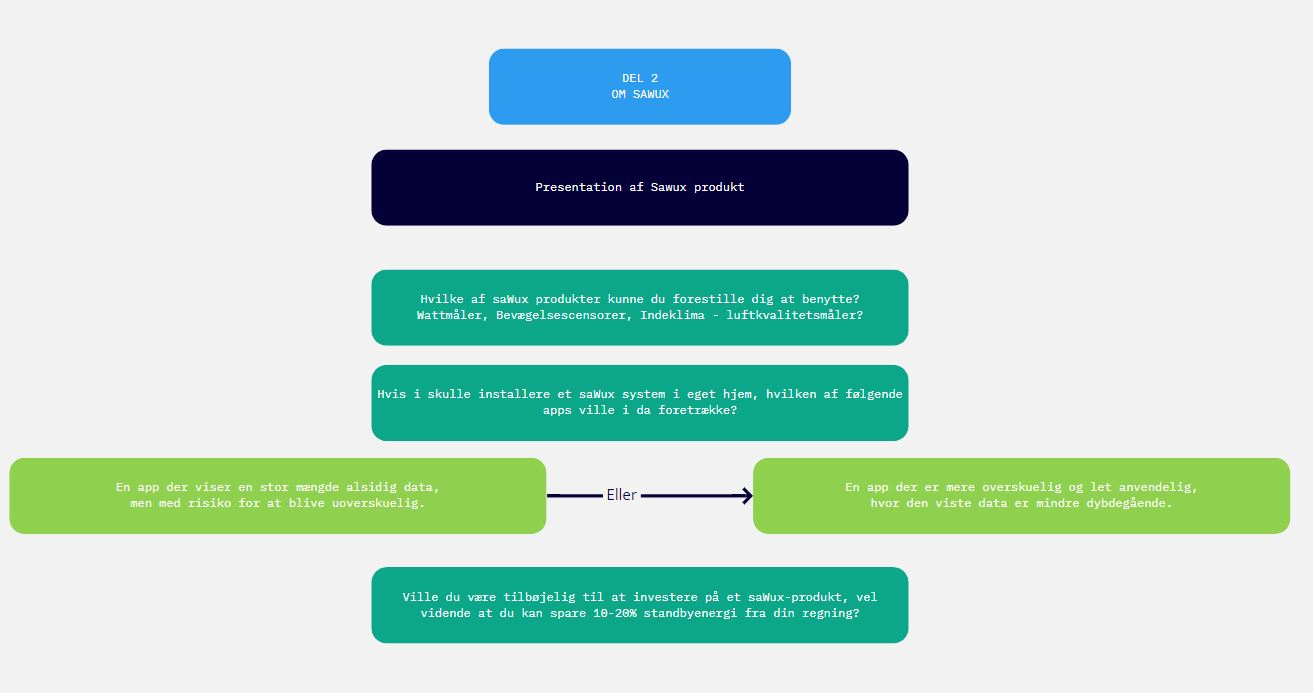
\includegraphics[width=\textwidth]{Images/appendixB/3.jpg}
    \caption{Kvalitativt interview guide — Del 3}
    \label{img:appendixc:3}
\end{figure}

\begin{figure}
    \centering
    
\includegraphics[width=\textwidth]{Images/appendixB/4.jpg}
    \caption{Kvalitativt interview guide — Del 4}
    \label{img:appendixc:4}
\end{figure}

\section{Opsummering}
Da vi ikke har mulighed for at have lydfiler som bilag vil dette bilag fungere som resultatet af vores kvalitative interview.

\subsection{Den Interviewede}
\textbf{Navn:} Camilla\\
\textbf{Køn og alder:} Kvinde, 31 år\\
\textbf{Rolle:} Mor til to. Bor med børn og mand.\\

\subsection{Vigtigste pointer fra interview}
\begin{itemize}
    \item Familien har ingen smart-home devices.
    \item De syntes det lyder meget attraktivt at investere i produkter der fremmer energistyring.
    \item De er specifikt interesserede i wattmåleren fra saWux.
    \item De ville foretrække en app der kan vise en stor mængde dybdegående data, men med mindre overskuelighed. (Frem for en simpel overskuelig app). 
    \item Familien er meget interesserede i det grønne aspekt af elbesparelse.
    \item De bruger i forvejen tid på at snakke om klima med børnene.
    \item Camilla syntes at det er en rigtig god idé med en app der inddrager familiens yngste medlemmer i energistyring.
\end{itemize}